\section{Rigid Body Kinetics}

\subsection{\red{Center of mass (COM)}}
\blue{Complete in "Center of mass"} 

\noindent \red{Add to this section the information shown in Fig \ref{fig:COM}}

\begin{figure}[h!]
    \centering 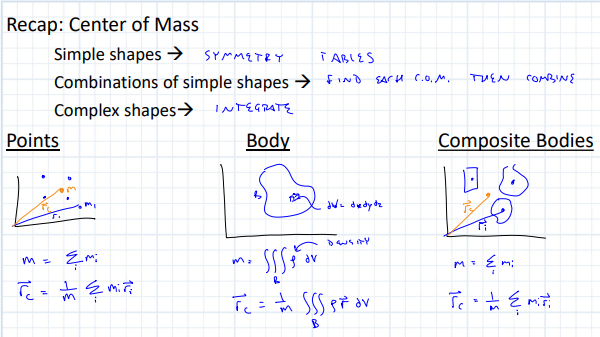
\includegraphics{RigidBodyKineticsFigs/CenterofMass.png}
    \caption{From L12-Notes, slide 2}
    \label{fig:COM}
\end{figure}

\subsection{Mass moment of inertia}
\blue{Complete in "Moments of Inertia"} 

\subsubsection{Parallel axis theorem}
\blue{Complete in "Moments of Inertia"} 
 
\subsubsection{Additive theorem}
\blue{Complete in "Moments of Inertia"} 

\subsection{\red{Instantaneous centers}}
\red{Add this information:}
\begin{itemize}
    \item \red{For a rigid body moving in 2D (rotating and possibly translating)}
    \item \red{Instantaneous Center “M” is the point on or off the rigid body that has zero
velocity at that instant (i.e. no translation at this point)}
    \item \red{Point that the body rotates about (at that instant in time)}

\end{itemize}

\red{Add some examples as shown in Figs \ref{fig:ICexamples1}, \ref{fig:ICexamples2}}

\begin{figure}[h!]
    \centering 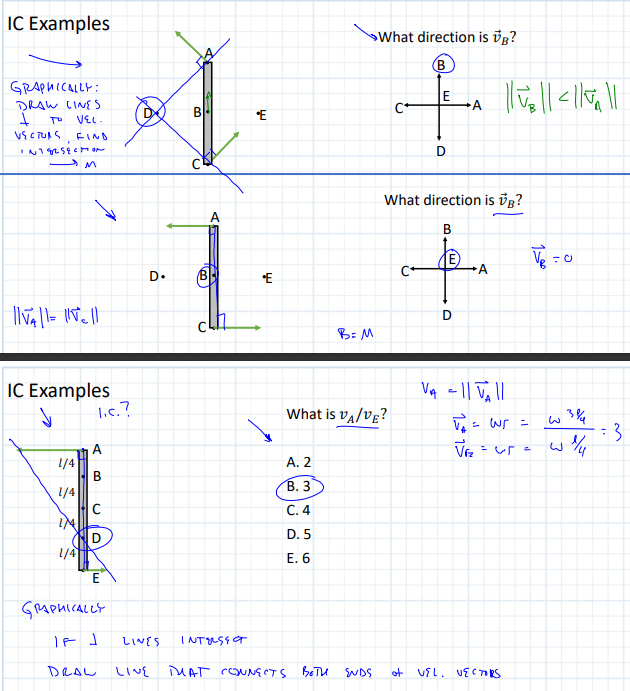
\includegraphics{RigidBodyKineticsFigs/ICexamples1.png}
    \caption{From L25-Notes, slides 5-6}
    \label{fig:ICexamples1}
\end{figure}

\begin{figure}[h!]
    \centering 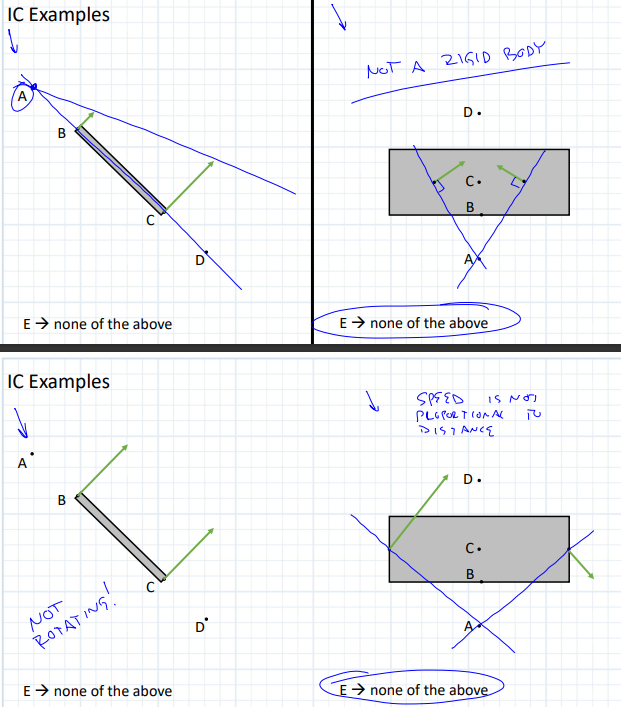
\includegraphics{RigidBodyKineticsFigs/ICexamples2.png}
    \caption{From L25-Notes, slides 8-9}
    \label{fig:ICexamples2}
\end{figure}

\red{Add: Graphical rules for finding (M) (Instantaneous Center) as shown in Fig\ref{fig:ICgraphRules}}

\begin{figure}[h!]
    \centering 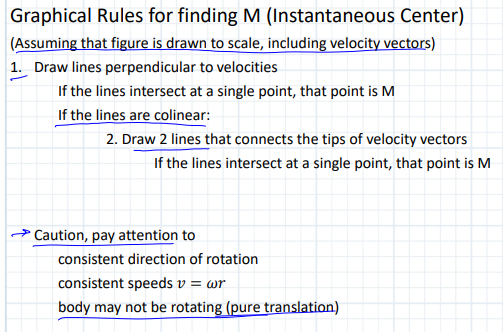
\includegraphics{RigidBodyKineticsFigs/ICgraphicalRules.png}
    \caption{From L25-Notes, slide 10}
    \label{fig:ICgraphRules}
\end{figure}

\subsection{\red{Applications}}
    \subsubsection{\red{Cargo Ships}}
    \red{This topic is in L22-Notes, slides 3-4, refer to Fig \ref{fig:AppCargoShip}}. Application for "Center of mass".

    \begin{figure}[h!]
        \centering
        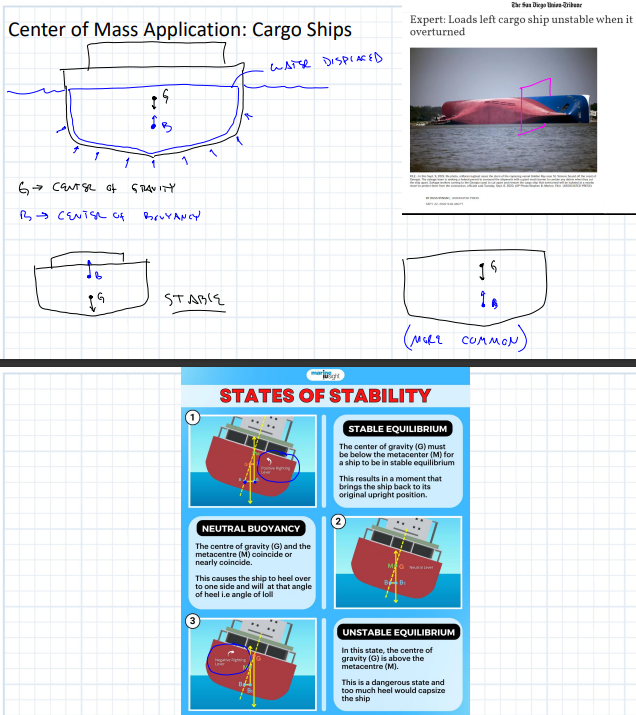
\includegraphics{RigidBodyKineticsFigs/AppCargoShip.png}
        \caption{From L22-Notes, slides 3-4.}
        \label{fig:AppCargoShip}
    \end{figure}

    \subsubsection{Tuned Mass Damper}
    \red{This topic is in L24-Notes, slide 9, include the information in Fig \ref{fig:AppCargoShip}, and this link to a YouTube video \url{https://www.youtube.com/watch?v=GzMuF-LMGaM} }. Application for "Rigid body kinetics".

    \begin{figure}[h!]
        \centering
        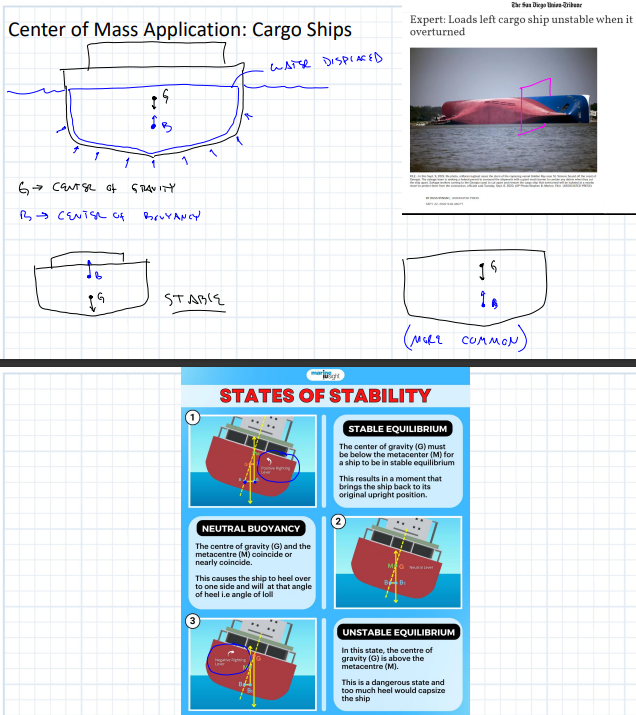
\includegraphics{RigidBodyKineticsFigs/AppCargoShip.png}
        \caption{From L24-Notes, slide 9.}
        \label{fig:AppCargoShip}
    \end{figure}

    \subsubsection{Accelerating and braking}
    \blue{Complete in "Accelerating and braking". Include all the information starting at "2D rigid body model".} Refer back to  \ref{sub:PartKin_acce}

    \subsubsection{Banked turns}
    \blue{Complete in "Banked turns". Include all the information starting at "2D rigid body model".} Refer back to  \ref{sub:PartKin_turns}